\documentclass[aspectratio=169]{beamer}
\usepackage{basileabeam}
\usepackage{epigraph}
\usepackage{graphicx}
\usepackage{multirow}
%\usepackage{enumitem}
\usepackage{array}
%\usepackage{multimedia}
\usepackage{media9}
%\usepackage{pdfpc-movie}
\usepackage{tikz}
\usepackage{listings}
\usepackage[normalem]{ulem}
%\usepackage{Sweave}
%\usepackage{xkeyval}
%\usepackage{palatino}
%\usepackage{pgfpages}
%\usepackage[font=Times,timeinterval=1, timeduration=200,resetatpages=all]{tdclock}
\usepackage[timeinterval=1]{tdclock}
%\usepackage[font=Times,timeinterval=10, timeduration=2.0, timedeath=0, fillcolorwarningsecond=white!60!yellow,timewarningfirst=50,timewarningsecond=80,resetatpages=2]{tdclock}
%*-------------------------------------------------------------------------------
%\newcolumntype{C}[1]{>{\centering\arraybackslash}m{#1}}
\newcolumntype{L}[1]{>{\raggedright\let\newline\\\arraybackslash\hspace{0pt}}m{#1}}
\newcolumntype{C}[1]{>{\centering\let\newline\\\arraybackslash\hspace{0pt}}m{#1}}
\newcolumntype{R}[1]{>{\raggedleft\let\newline\\\arraybackslash\hspace{0pt}}m{#1}}
%*-------------------------------------------------------------------------------
%\pgfpagesuselayout{2 on 1}[a4paper,border shrink=5mm]
%\setbeamertemplate{note page}[plain]
%\setbeameroption{show notes on second screen=bottom}
%*-------------------------------------------------------------------------------
\setbeameroption{hide notes}
%\setbeameroption{show only notes}
%\setbeameroption{show notes on second screen=right}
\setbeamertemplate{note page}{\pagecolor{yellow!5}\insertnote}
%*-------------------------------------------------------------------------------
\title              {Programa de formação em Robótica - Desafio 2.5}
\author             {Marco Reis}
\email              {marcoreis@me.com}
\institute          {Laboratório de Robótica e Sistemas Autônomos, Senai Cimatec}
\date               {Abril de 2020}
\ulogo        		{Template/logosenaicimatec}
\ulogoo        		{Template/fibonacci}
\ulistelement    	{Template/sunflower}
%*-------------------------------------------------------------------------------
\graphicspath{{Media/pictures/}}
%*-------------------------------------------------------------------------------
\totalNoSlidesDisabled % To turn off the total number of slides in the footer. Comment this if you want the total number of slides in the footer
%*-------------------------------------------------------------------------------
\begin{document}
%*----------- COVER -------------------------------------------------------------
 \begin{frame}[t,plain]
%*----------- sound
    \includemedia[
        %width=1ex,
        %height=1ex,
        activate=pageopen, 
        deactivate=onclick,
        %passcontext,
        transparent,
        addresource=./Media/sounds/loop-mix.mp3,
        flashvars={
                    source=./Media/sounds/loop-mix.mp3
                    %&autoPlay=true
                    &autoRewind=true
                    &Play=2s
                    &repeat=always
                    %&Loop=true
                }
                ]
    {}{VPlayer.swf}
%*----------- start-page
    \titlepage
%*----------- notes
    \note[item]{Notes can help you to remember important information. Turn on the notes option.}
    \note[item]{Notes can help you to remember important information. Turn on the notes option.}
\end{frame}
%-
%*----------- SECTIONS ----------------------------------------------------------
%*----------- SLIDE -------------------------------------------------------------
\begin{frame}[t]{Introdução} 
    \transdissolve[duration=0.5]
    Um dos pontos importantes na área da robótica é a interação entre os sistemas, e em decorrência ao programa de formação em robótica uma das lacunas será preenchida com o desenvolvimento do desafio 2.5..

    O desafio consiste em:
    %\newline
        \begin{columns}[t]
            \column{.05\linewidth}
            \column{.4\linewidth}
                \begin{enumerate}
                    \item assimilar o conhecimento da interação em robots;
                    \item compreender em profundidade os conceitos de simulação, e o;
                    \item desenvolvimento da liderança em projetos.
                \end{enumerate}
            \column{.6\linewidth}
            \begin{center}
            %\centerline{
                \begin{figure}
                    %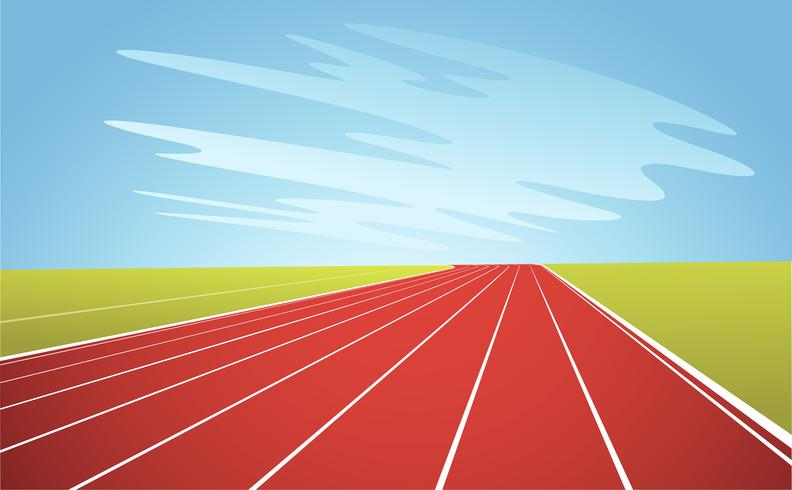
\includegraphics[width=1\textwidth]{pista}
                    \caption{Pista de corrida \cite{agostini2007}}
                    \roundpic[xshift=0cm,yshift=0cm]{4cm}{7cm}{pista}
                    %\caption{Pista de corrida \cite{agostini2007}}
                \end{figure}
            %}
            \end{center}
        \end{columns}
%*----------- notes
    \note[item]{Notes can help you to remember important information. Turn on the notes option.}
\end{frame}
%-
%*----------- SLIDE -------------------------------------------------------------
\begin{frame}[t]{O sistema robótico}
    \transboxout[duration=0.5]
    \begin{columns}
        \column{.1\textwidth}
        \column{.4\textwidth}
            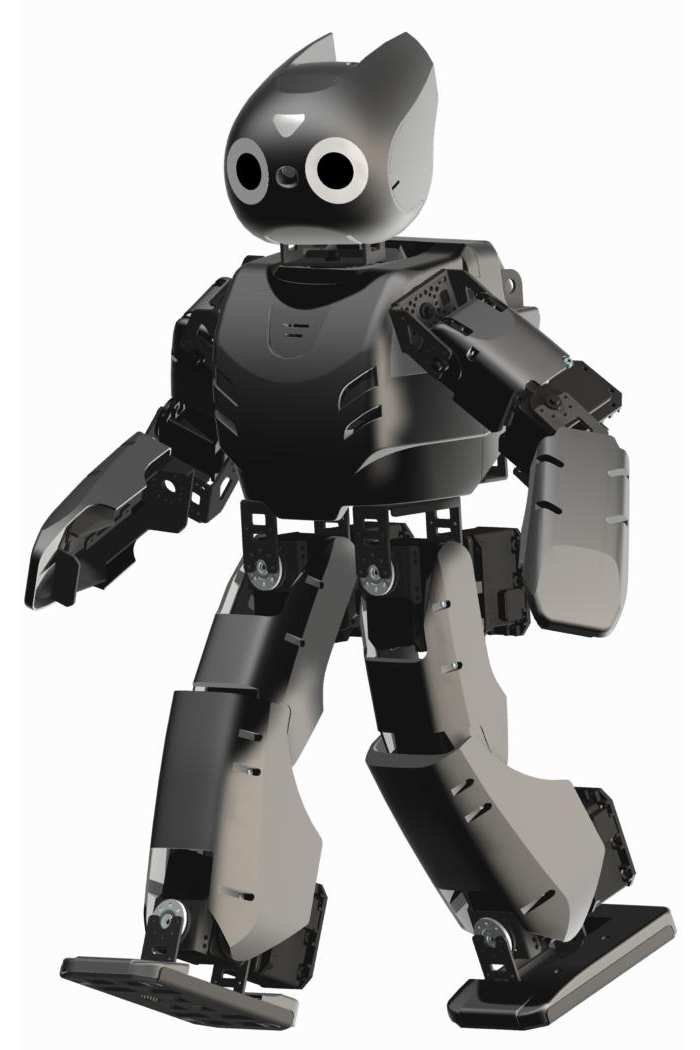
\includegraphics[width=.8\textwidth]{darwin-op}
        \column{.4\textwidth}
            \begin{enumerate}
                \item plataforma antropormórfica Darwin-OP;
                \item 20 DoF\footnote{do inglês, graus de liberdade};
                \item composto de 18 servo-motores;
                \item possui um grande gama de sensores para interação.
            \end{enumerate}
    \end{columns}
%*----------- notes
    \note[item]{Notes can help you to remember important information. Turn on the notes option.}
\end{frame}
%-
%*----------- SLIDE -------------------------------------------------------------
\begin{frame}[c]{Darwin-OP - overview}
    %\transboxin[duration=1,direction=30]
    \centering
    %   \movie[width=12.8cm,height=7.2cm,showcontrols=true,poster,autostart]
    %         {\includegraphics[width=12.8cm,height=7.2cm]{Darwin-OP}}
    %         {Darwin-OP.mp4}


          %Videos and audios don't play on Overleaf! Download the PDF and open in Acrobat Reader to view. :-)

          %This is an .mp4 file:
          
          % using a .mp4; downloaded from https://www.youtube.com/watch?v=-9iXD2-hbJM
          %\includemedia[width=0.6\linewidth,height=0.6\linewidth,activate=pageopen,passcontext,transparent,addresource=penguinschasingbutterfly.mp4,flashvars={source=penguinschasingbutterfly.mp4}]{\includegraphics[width=0.6\linewidth]{penguins}}{VPlayer.swf}
          
          %This is a YouTube video (needs an Internet connection to view):
          
          % using a YouTube video
         % \includemedia[width=0.6\linewidth,height=0.3375\linewidth,activate=pageopen,flashvars={modestbranding=1 &autohide=1 autohide &showinfo=0 &rel=0}]{\includegraphics[width=0.6\linewidth]{Darwin-OP}}{https://www.youtube.com/v/g8Ejj0T0yG4?rel=0}
          
          %This is an .mp3 file:
          %% MP3 downloaded from https://www.sample-videos.com/download-sample-audio.php
        %   \includemedia[transparent,passcontext,addresource=SampleAudio.mp3,flashvars={source=SampleAudio.mp3},]{\color{blue}\framebox[0.4\linewidth][c]{Applause}}{APlayer.swf}

    \includemedia[
      width=0.7\linewidth,
      totalheight=0.39375\linewidth,
      activate=pageopen,
      passcontext, 
      addresource=./Media/movies/Darwin-OP.mp4,
      flashvars={
      source=./Media/movies/Darwin-OP.mp4
      &autoPlay=true
      &Loop=false}
      ]{\fbox{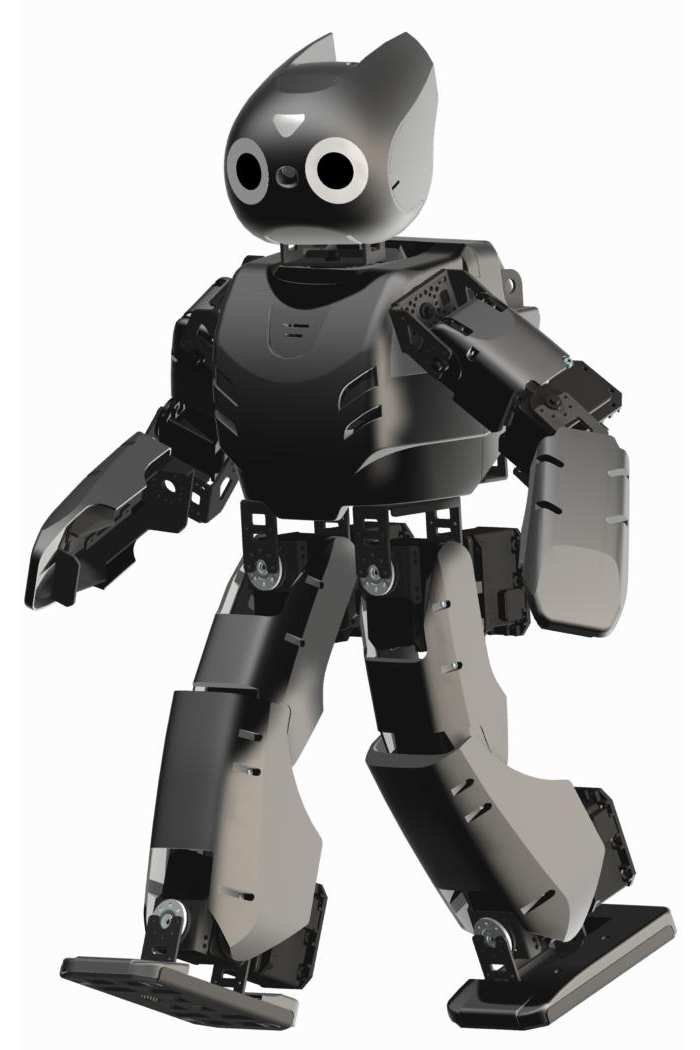
\includegraphics{darwin-op}}}{VPlayer.swf}

    %    \includemedia[
    %      width=0.4\linewidth,
    %      totalheight=0.225\linewidth,
    %      activate=pageopen,
    % %     passcontext,  %show VPlayer's right-click menu
    % %     addresource=Figures/Darwin-OP.mp4,
    %      flashvars={
    % %     %important: same path as in `addresource'
    % %     source=Figures/Darwin-OP.mp4}
    %         modestbranding=1 % no YT logo in control bar
    %         &autohide=1 % controlbar autohide
    %         &showinfo=0 % no title and other info before start
    %         &rel=0 % no related videos after end
    %         }
    %     ]{}{http://www.youtube.com/embed/1WEgNQjL66g}
    % %     &autoPlay=true
    % %     &Loop=false}
    % %     ]{\fbox{Click!}}{VPlayer.swf}

    %\pdfpcmovie{\includegraphics[width=.3\textwidth]{Darwin-OP}}{Darwin-OP.mp4}
%*----------- notes
    \note[item]{Notes can help you to remember important information. Turn on the notes option.}
\end{frame}
%-
%*----------- SLIDE -------------------------------------------------------------
\begin{frame}[c]{A tropa dos quatro incríveis}
    %\transboxin[duration=1,direction=30]
    A simulação deverá ser desenvolvida com 4 unidades Darwin-OP, comumente esta unidade é utilizada para desafios em competições de robótica.
    \newline

    A tropa será composta por 4 Darwin-OP, e deverá realizar duas missões:
    \begin{itemize}
        \item marchar em forma unida em linha;
        \item realizar corrida de revezamento.
    \end{itemize}

    \begin{figure}
        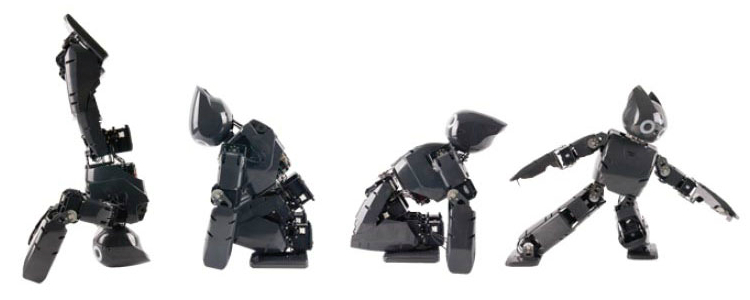
\includegraphics[width=0.8\textwidth]{darwin-op-sequencia}
        %\caption{.}
    \end{figure}
%*----------- notes
    \note[item]{Notes can help you to remember important information. Turn on the notes option.}
\end{frame}
%-
%*----------- SLIDE -------------------------------------------------------------
\begin{frame}[t]{Algumas regras}
    \begin{itemize}
        \item A marcha deverá ser realizada diante de um percurso de 2 metros.
        \item A marcha e a corrida de revezamento deverão serem realizadas numa pista de corrida;
        \item A corrida deverá ser realizada numa pista de 8 metros;
        \item Cada Darwin-OP deverá percorrer 2 metros para realizar o revezamento;
        \item A região de revezamento deverá ser uma área de até 0.4 metros;
        \item O conceito para o revezamento será o de alinhar-se os dois Darwin-OP durante até 15 segundos a uma distância de no máximo 0.2 metros entre ambos, ou seja será considerado passagem de bastão quando os dois Darwin-OP passarem 15 segundos com movimentos sincronizados a uma distância máxima de 0.2 metros dentro da região de revezamento;
        \item A pista de corrida deverá ser considerada analogamente a uma pista real;
        \item A lateral da pista deverá ter lados de 2 metros;
        \item Considerar sempre os critérios de uma corrida de revezamento.
        \item askjfdaslkjfdslak
    \end{itemize}
   
    % \begin{columns}[t]
    %     \column{.45\textwidth}
    %         detalhar sistemas em subconjuntos\\
    %         listar possíveis modos de falhas\\
    %         analisar cada modo de falha, juntamente com suas possíveis causas e sintomas
    %     \column{.45\textwidth}
    %         estimar os efeitos de cada modo de falhas\\
    %         estimar a criticidade de cada efeito\\
    %         identificar ações para minimizar falhas
    % \end{columns}
%*----------- notes
    \note[item]{Notes can help you to remember important information. Turn on the notes option.}
\end{frame}
%-
%*----------- SLIDE -------------------------------------------------------------
\begin{frame}[c]{A pista}
    \begin{figure}
        %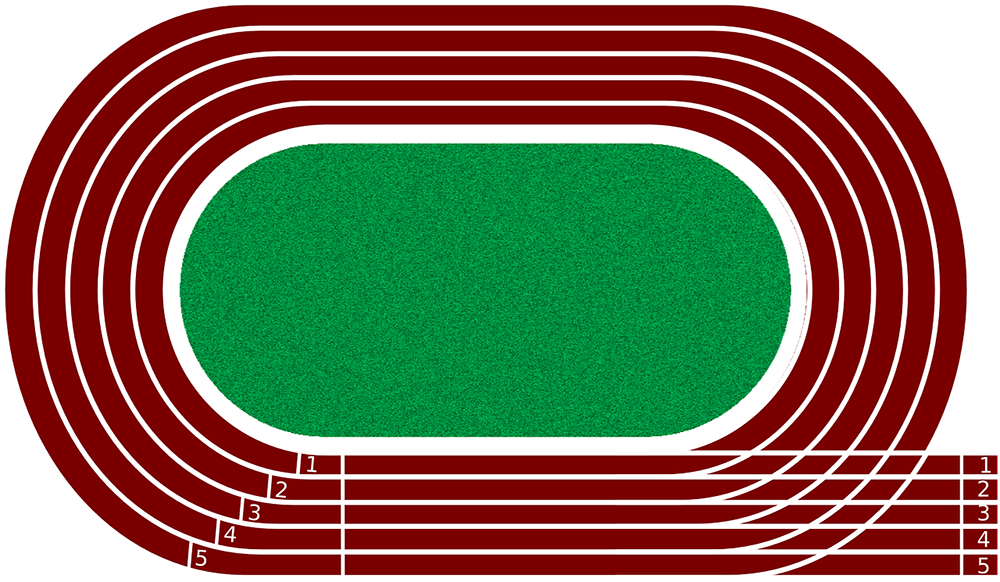
\includegraphics[width=0.7\textwidth]{pista_corrida}
       
        \roundpic[xshift=0cm,yshift=0cm]{2.8cm}{3cm}{pista_corrida}
          
        \caption{Formato de um pista de corrida.\cite{agostini2007}}
    \end{figure}
%*----------- notes
    \note[item]{Notes can help you to remember important information. Turn on the notes option.}
\end{frame}
%-
%*----------- SLIDE -------------------------------------------------------------
\begin{frame}[t]{As lideranças das equipes dos Novos Talentos}
    \vspace{0.5cm}
    \begin{columns}
        \column{.01\textwidth}
        \column{.7\textwidth}
            \begin{itemize}
                \item equipe RAJA será liderada por Aziel Freitas
                \item equipe BORG será liderada por Mateus Cerqueira.
                \item equipe TIMON-HM será liderada por Leonardo Lima.
            \end{itemize}
        \column{.29\textwidth}
            
\includegraphics[width=.9\textwidth, trim={10cm 0 10cm 0},clip]{equipe}
    \end{columns}
    \vspace{1cm}
    
    \emph{Para este desafio não será cobrado o relatório técnico, porém o acompanhamento deverá seguir o mesmo ritmo dos desafios anteriores.}
%*----------- notes
    \note[item]{Notes can help you to remember important information. Turn on the notes option.}
\end{frame}
%-
%*----------- SLIDE -------------------------------------------------------------
\begin{frame}[t]{O progresso das equipes}
    Um dos indicadores para o acompanhamento das equipes será o percentual de conclusão geral da equipe.
    O planejamento das atividades deverá seguir a metodologia aplicada no desenvolvimento de projetos de robótica.
    \newline
    %\vspace{0.5cm}
    \begin{table}[ht!]
    \centering
        \caption{PERCENTUAL DE CONCLUSÃO POR EQUIPE}
        \begin{tabular}{|l|c|c|c|c|} \hline
            \textbf{EQUIPE}&\textbf{04/05}&\textbf{11/05}&\textbf{18/05}&\textbf{25/05}\\ \hline
            RAJA & 17\% &32\% & &  \\ \hline
            BORG & 0\% &41\% & &  \\ \hline
            TIMON-HM & 5\% &47\% & &  \\ \hline
        \end{tabular}
    \end{table}
%*----------- notes
    \note[item]{Notes can help you to remember important information. Turn on the notes option.}
\end{frame}
%-
%*----------- SLIDE -------------------------------------------------------------
\begin{frame}[t]{Finalização}
    \begin{itemize}
        \item Cada líder deverá realizar a apresentação final do desafio no dia 15/maio/2020.
        \item No dia da apresentação, somente o líder poderá responder os questionamentos emitidos pelos facilitadores.
        \item A avaliação será da equipe, não havendo avaliação individual dos integrantes da equipe com exceção do líder de cada equipe.
        \item A apresentação deverá ser desenvolvida em latex.
        \item Os videos dos desafios deverão estar contidos na apresentação final.
        \item Os videos deverão ser completos, tendo começo, meio e fim da missão realizada.
    \end{itemize}
%*----------- notes
    \note[item]{Notes can help you to remember important information. Turn on the notes option.}
\end{frame}
%-
%*----------- SLIDE -------------------------------------------------------------
\begin{frame}[c]{A importância atual da robótica}
    \begin{center}
        % \movie[loop,width=0.6\linewidth,height=0.3375\linewidth,showcontrols=false,autostart]{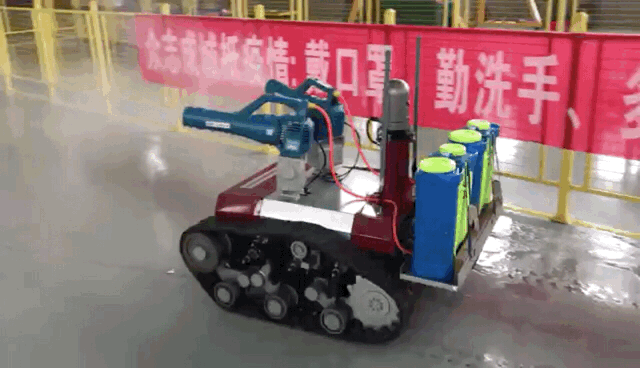
\includegraphics[width=0.6\textwidth]{Media/gifs/robotdesinfec0.png}}{Media/gifs/robotdesinfec.wmv}
    
        \includemedia[
            width=0.7\linewidth,
            totalheight=0.39375\linewidth,
            activate=pageopen,
            passcontext, 
            %transparent,
            addresource=./Media/gifs/robotdesinfec.wmv,
            flashvars={
            source=./Media/gifs/robotdesinfec.wmv
            &autoPlay=true
            &autoRewind=true
            &loop=true}
            ]{\fbox{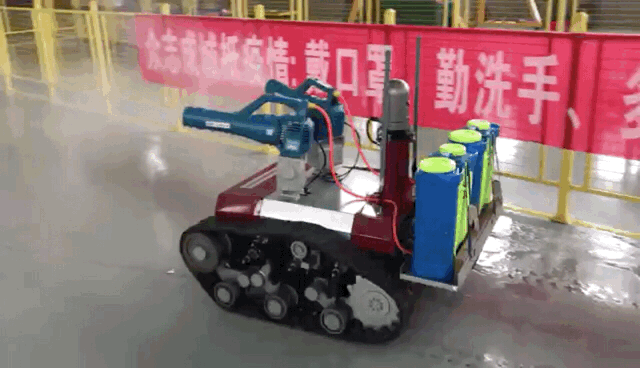
\includegraphics{Media/gifs/robotdesinfec0.png}}}{VPlayer.swf}
    \end{center}
%  %\movie[width=8cm,height=4.5cm]{test}{../Movies/Darwin-OP.mp4}

% % \includemedia[
% %     width=0.4\linewidth,
% %     totalheight=0.225\linewidth,
% %     activate=pageopen,
% %     passcontext,  %show VPlayer's right-click menu
% %     addresource=../Movies/Darwin-OP.mp4,
% %     flashvars={
% %       %important: same path as in `addresource'
% %       source=../Movies/Darwin-OP.mp4
% %     }
% %   ]{\fbox{Click!}}{VPlayer.swf}

%     \pdfpcmovie{\includegraphics[width=\textwidth]{Darwin-OP}}{Darwin-OP.mp4}

%*----------- notes
    \note[item]{Notes can help you to remember important information. Turn on the notes option.}
 \end{frame}
 %-
%-
%*----------- SLIDE-BACKUP ------------------------------------------------------
% \backupbegin
% %
% \begin{frame}{Backup}
%     Test
% %*----------- notes
% \note{Notes can help you to remember important information. Turn on the notes option.}
% \end{frame}
% %-
% \backupend
% %-
%*----------- QUESTIONS ---------------------------------------------------------
\begin{frame}[t,plain]
    \lastpage{{\usebeamerfont{title} Questions?}\\[3ex] \hspace{0.1cm} marcoreis@me.com}
%*----------- notes
    \note[item]{Notes can help you to remember important information. Turn on the notes option.}
\end{frame}
%-
\end{document}